\documentclass[pscyr]{hedlab}
\usepackage[russian]{babel}
\usepackage{graphicx}
\graphicspath{{images/}}
\usepackage{listings}

\lstset{
    basicstyle=\footnotesize,
    inputencoding=utf8,
    extendedchars=True,
    language=[Sharp]C,
    numbers=left,
    numberstyle=\footnotesize,
    breakatwhitespace=\false,
    breaklines=True,
    tabsize=2,
    keepspaces=true,
}

\labname{Аутентификация и авторизация в Web-приложениях}
\labnum{6}
\student{Чечеткин И. А., САПР-1.1п}
\labdate{}

\begin{document}
    \makeheader
    \emph{Цель:} получение практических навыков создания безопасных ASP.NET приложений с 
    использованием механизмов аутентификации и авторизации.
    
    \emph{Задача:} создать ASP.NET приложение, осуществляющее аутентификацию
      пользователя, и настроить web.config файл в соответствии с заданием.

    Для создания аутентификации была использована библиотека Owin.
    
    \lstinputlisting[language=HTML,title={Страница авторизации:}]{code/login.aspx}
    
    \lstinputlisting[title={Код авторизации:}]{code/login.cs}
    
    \lstinputlisting[title={Код регистрации:}]{code/register.cs}

    \lstinputlisting[title={Конфигурация:}]{code/startup.cs}

    \pagebreak

    \begin{figure}[h!]
        \center
        Скриншоты Web-страниц:\\
        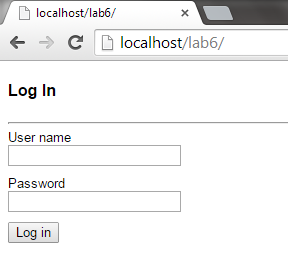
\includegraphics[height=12em]{01} \hspace{.5em}
        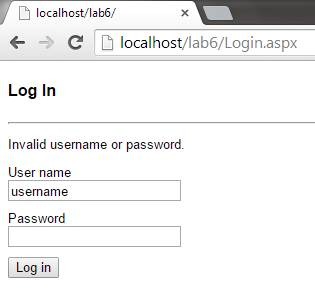
\includegraphics[height=12em]{03} \hspace{.5em}
        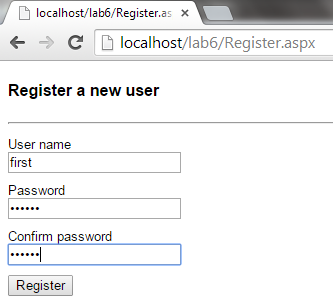
\includegraphics[height=12em]{04} \\
        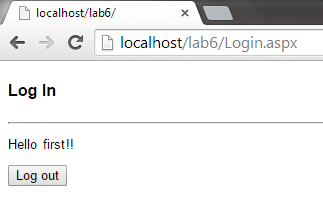
\includegraphics{02}
    \end{figure}

    \emph{Вывод:} в результате проделанной работы создал ASP.NET приложение,
      осуществляющее аутентификацию пользователя, и настроил web.config файл
      в соответствии с заданием.
\end{document}